\documentclass[10pt,twocolumn]{article}

\usepackage[margin=1.85cm,columnsep=0.6cm]{geometry}
\usepackage{mathptmx}
\usepackage[T1]{fontenc}
\usepackage{graphicx}
\usepackage{booktabs}
\usepackage{caption}
\usepackage{amsmath}
\usepackage{xcolor}
\usepackage[colorlinks=true,linkcolor=blue!50!black,citecolor=blue!50!black,urlcolor=blue!50!black]{hyperref}
\usepackage{titlesec}
\usepackage{enumitem}

\setlength{\parskip}{2pt}
\setlength{\abovecaptionskip}{3pt}
\setlength{\belowcaptionskip}{-4pt}
\titlespacing*{\section}{0pt}{7pt}{4pt}
\titlespacing*{\subsection}{0pt}{5pt}{2pt}
\captionsetup{font=small,labelfont=bf}

\newcommand{\tcd}{\ensuremath{\mathrm{TCD}}}

\title{\vspace{-1.2em}\textbf{Does Network Topology Change Which Policy Wins?\\
\large A Paired-Simulation Evaluation of a Bounded LLM Agent Against a Classical Heuristic Under Supply-Chain Disruption}}
\author{\small Yassine Erraji \\[-2pt] \small \texttt{supply-chain-agent-evaluation}, Version 2}
\date{\small August 2026}

\begin{document}
\maketitle
\vspace{-1.8em}

\begin{abstract}
\noindent We evaluate whether a bounded, tool-using LLM agent makes cheaper shipment-routing decisions than a transparent cost-minimizing heuristic under supply-chain disruption, using a discrete-time simulator with a strict paired-replication design. A first version (V1) found the LLM agent winning overwhelmingly under Medium/Heavy disruption and losing under Light disruption -- but with an unusual property: all 300 replications, across three severities, agreed unanimously (100\%/0\% win rate in every profile). An audit attributed this to insufficient randomness and a single, low-redundancy network topology, not to a genuine effect ceiling. Version 2 (V2) crosses three network topologies (Compact/Standard/Extended, varying route redundancy from zero to seven non-emergency paths) against three disruption severities, and adds per-replication randomness to disruption timing, duration, disclosure delay, and shipment volume. Across all nine live-API cells (498 total replications), every cell's 95\% confidence interval excludes zero, and one cell produces a genuinely mixed outcome (75.8\% LLM win rate) for the first time in either version of this project. The central finding is that \textbf{topology does not merely scale the LLM's advantage -- it reverses its sign}: on the two lower-redundancy topologies the LLM's advantage grows with severity, while on the highest-redundancy topology the heuristic's advantage grows with severity instead.
\end{abstract}

\section{Research Problem}
\label{sec:intro}
LLM-based agents are increasingly proposed for operational decisions -- rerouting, expediting, cancelling shipments -- where a wrong call has a directly measurable cost. Most public demonstrations of ``AI beats the baseline'' in this space do not survive scrutiny: mismatched scenarios, cherry-picked examples, or a classical baseline that was never given a fair, symmetric shot. This work isolates one narrow, well-defined decision -- \emph{what should happen to a shipment sitting at a node when the surrounding network is disrupted} -- and asks: \textbf{under identical disrupted conditions and identical operational constraints, can a bounded LLM policy reduce the incremental cost of disruption more effectively and more robustly than a transparent classical heuristic, and how does that advantage depend on network structure and disruption severity?}

Fairness is operationalized structurally rather than asserted: both policies observe the same read-only state, are validated and fall back through the same machinery, and face the same stochastic demand, delay, and disruption realization within a replication. Each policy is scored against its own undisrupted counterfactual, never against the other policy's raw cost -- isolating the \emph{incremental} cost of disruption, not baseline operating cost.

\section{Related Work}
\label{sec:relwork}
\textbf{LLM agents with tools.} The ReAct paradigm \cite{yao2022react} established the now-standard architecture for LLM agents: an interleaved reasoning--action--observation loop, later made reliable via structured function calling. Toolformer \cite{schick2023toolformer} showed LLMs can learn when to invoke external tools rather than merely being prompted to. Our agent follows this lineage directly: five deterministic, read-only tools, an 8-call budget, temperature 0, and a hard fallback to the classical heuristic on abstention or invalid output.

\textbf{LLM agents in supply chain management.} Applying LLM agents to logistics and supply-chain decisions is an active, recent research direction. InvAgent \cite{invagent2024} applies multi-agent LLMs to inventory management under demand uncertainty; broader surveys \cite{llmscm2025} catalog knowledge-integration and multi-agent negotiation as the dominant use cases; \cite{agenticscm2025} studies LLM agents reaching autonomous consensus across supply-chain roles. This literature consistently flags a verification gap: agentic LLMs can inherit human-like biases and produce confidently wrong decisions absent explicit checking -- precisely the concern our validator-and-fallback layer exists to close, and precisely the reason this study reports null and negative results (Section~\ref{sec:results}) alongside positive ones rather than only the favorable cells.

\textbf{Classical disruption management.} The heuristic baseline sits in a long tradition of cost-minimizing routing and inventory-recovery rules under disruption \cite{sheffi2005resilient,christopher2004building}: transparent, auditable, and structurally incapable of considering information outside its candidate-route cost estimate. We do not treat it as a strawman -- V1 already showed it winning cleanly under Light disruption, and V2's Extended topology shows it winning at every severity.

\section{Methodology}
\label{sec:method}
\textbf{Simulator.} A discrete-time (daily), single-product simulator over a directed logistics network (suppliers~$\to$~ports~$\to$~hubs~$\to$~plant). A policy intervenes on at most one shipment per decision point with exactly one action: \texttt{WAIT}, \texttt{REROUTE}, \texttt{EXPEDITE}, or \texttt{ABSTAIN}; every proposed action passes a shared validator before being applied, with a heuristic-then-\texttt{WAIT} fallback chain on failure.

\textbf{Paired protocol.} One random seed drives one \emph{replication}: a shared draw of demand, ordinary transport delay, and (in V2) disruption realization and shipment volume, generated entirely before either policy acts. From this one draw, four cloned branches run -- \{heuristic, LLM\}~$\times$~\{undisrupted, disrupted\} -- sharing an identical 20-day warm-up snapshot. Per policy $p$, $\tcd_p = J^{\text{disrupted}}_p - J^{\text{undisrupted}}_p$, where $J$ sums transport, reroute, expedite, holding, backlog, late, and terminal costs. The reported effect is $\Delta = \tcd_{\text{LLM}} - \tcd_{\text{heuristic}}$ ($\Delta<0$ favors the LLM). This pairing removes common-mode noise (the same random world hits both policies), giving far more statistical power per replication than an unpaired comparison would.

\textbf{Why V2.} V1 ran one topology (5 nodes, 6 edges, $\sim$3 routes) against three severities, 100 replications each. Every profile's win rate was exactly 0\% or 100\%, and the mean $|\Delta|$ was $7.6\times$--$10.2\times$ larger than the between-replication standard deviation of $\Delta$ -- the environment could not generate a world where the effect and the noise were remotely comparable in scale. V2 targets this directly: (i) three topologies (Compact: 4~nodes/4~edges/0 non-emergency reroutes; Standard: V1's original network, unchanged; Extended: 10~nodes/16~edges/7 structurally distinct non-emergency routes, verified by betweenness centrality), crossed with the same three severities; (ii) disruption start day, duration, and disclosure delay now sampled per replication (a zero-uncertainty template provably reproduces V1 bit-for-bit); (iii) shipment quantity sampled per release on Compact/Extended (Standard keeps V1's fixed 40 units by design, as an unmodified behavioral anchor -- see Section~\ref{sec:limits}).

\section{Experimental Design}
Nine cells (3 topologies $\times$ 3 severities), each a flat, independently-run configuration -- no new orchestration layer. Compact and Extended run 33 replications/cell (base seed 2042/3042); Standard runs V1's original 100 replications/cell (seed 1042, unchanged) as the reference column. Extended's severity scenarios target \texttt{hub\_1} rather than \texttt{port\_primary}, since centrality analysis showed the latter is no longer the tier's structural chokepoint once seven alternate routes exist. All nine cells were first calibrated (3 replications each) before committing to the full run; the full grid then executed live against the OpenAI API (498 replications, $\sim$14{,}700 LLM calls, $\sim$4.5\,h wall-clock across three concurrent per-topology processes), all nine completing without error.

\section{Results}
\label{sec:results}
\begin{table}[t]
\centering
\small
\begin{tabular}{@{}llrrr@{}}
\toprule
Topology & Severity & Mean $\Delta$ & 95\% CI & LLM win \\
\midrule
Compact  & Light  & $+935$ & [814, 1055]      & 0\% \\
Compact  & Medium & $-1{,}436$ & [$-$2210, $-$663] & \textbf{75.8\%} \\
Compact  & Heavy  & $-56{,}915$ & [$-$68896, $-$44934] & 100\% \\
Standard & Light  & $+921$ & [857, 985]        & 0\% \\
Standard & Medium & $-4{,}192$ & [$-$4682, $-$3702] & 100\% \\
Standard & Heavy  & $-111{,}850$ & [$-$122960, $-$100741] & 100\% \\
Extended & Light  & $+1{,}636$ & [1451, 1820]    & 0\% \\
Extended & Medium & $+5{,}176$ & [4536, 5817]    & 0\% \\
Extended & Heavy  & $+22{,}114$ & [17950, 26279]  & 0\% \\
\bottomrule
\end{tabular}
\caption{Mean $\Delta$ (currency units; negative favors the LLM) and 95\% CI on all nine cells. $n=33$ for Compact/Extended, $n=100$ for Standard. Every CI excludes zero.}
\label{tab:grid}
\end{table}

Table~\ref{tab:grid} and Figure~\ref{fig:interaction} give the full grid. Compact and Standard replicate V1's shape: the heuristic wins Light, the LLM's advantage grows monotonically to a large, decisive win by Heavy. \textbf{Extended inverts this relationship}: the heuristic's advantage grows monotonically with severity instead, winning every replication at every severity. Topology is not a magnitude dial on a fixed direction of effect -- it can flip which policy is favored as conditions worsen.

\begin{figure}[t]
\centering
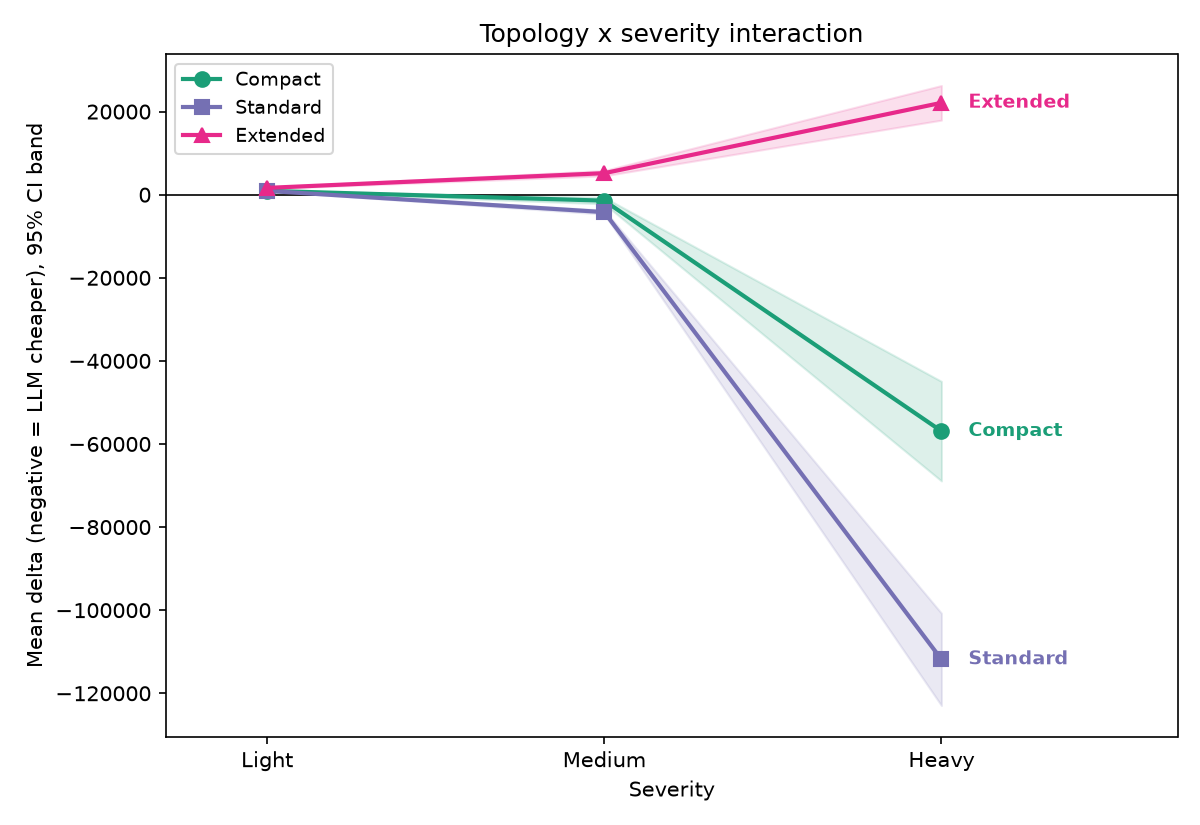
\includegraphics[width=\linewidth]{analysis/plots/v2_grid_full/grid/12_topology_severity_interaction.png}
\caption{Mean $\Delta$ vs.\ severity, one line per topology (signed-sqrt axis; shaded bands are 95\% CI). Compact and Standard diverge negative (LLM-favorable); Extended diverges positive (heuristic-favorable).}
\label{fig:interaction}
\end{figure}

Compact~$\times$~Medium is the one cell in either project version to land away from unanimity (75.8\% LLM, 24.2\% heuristic), direct evidence that V2's added randomness produces genuine per-replication variation rather than a foregone conclusion. Consistent with this, the signal-to-noise ratio $|\overline{\Delta}|/\mathrm{sd}(\Delta)$ sits at 0.6$\times$--3.0$\times$ across all nine V2 cells, against 7.6$\times$--10.2$\times$ recomputed identically on V1's original three real 100-replication runs -- the audited root cause is measurably fixed, not merely asserted fixed.

\begin{figure}[t]
\centering
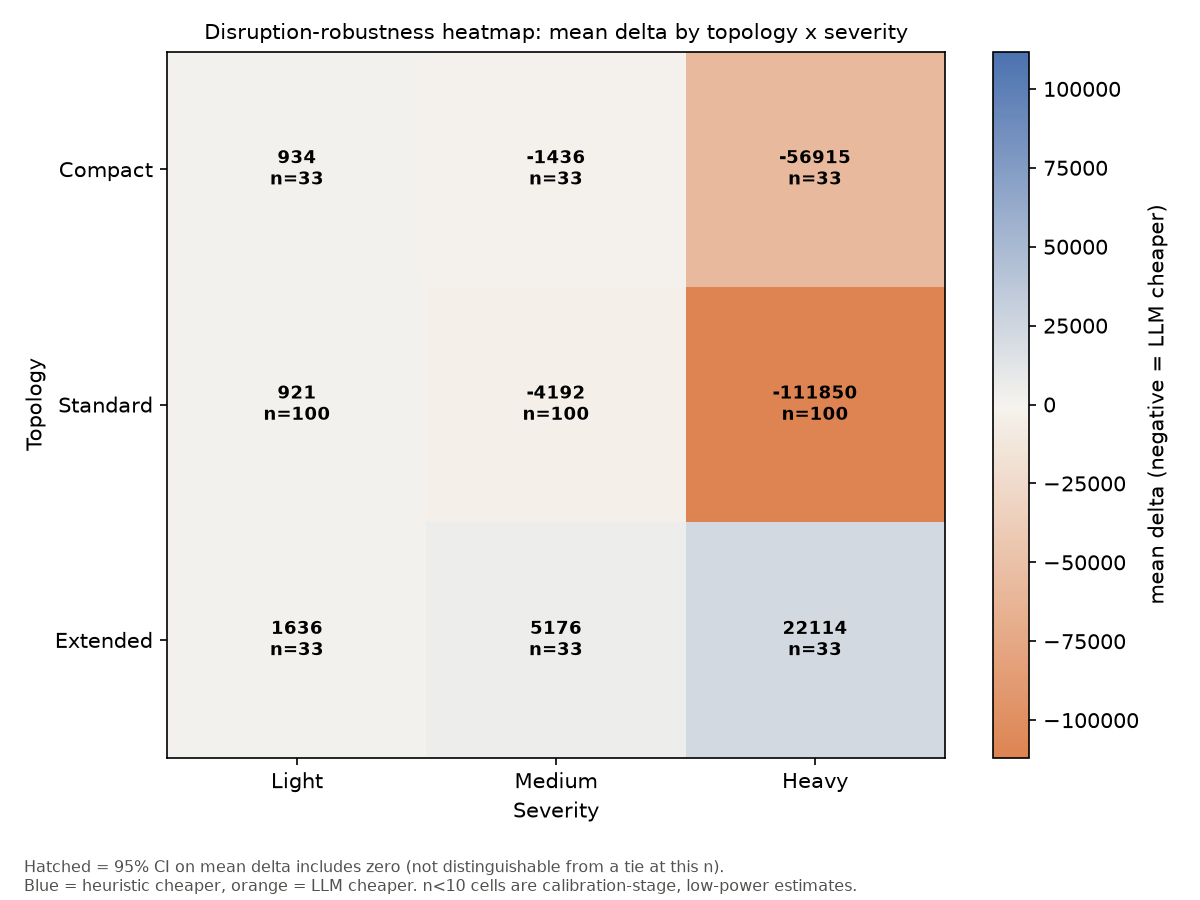
\includegraphics[width=\linewidth]{analysis/plots/v2_grid_full/grid/08_disruption_robustness_heatmap.png}
\caption{Mean $\Delta$ across the full grid (diverging color; orange = LLM-favorable, blue = heuristic-favorable). No cell is hatched -- every 95\% CI excludes zero, so all nine effects shown are real at this sample size, not noise.}
\label{fig:heatmap}
\end{figure}

\section{Discussion}
\textbf{Why might Extended reverse?} The heuristic exhaustively scores every candidate route by estimated cost and never has to judge which of many plausible options is worth pursuing; with seven real alternatives, that cheap, complete search may simply out-compete a bounded agent (max 8 tool calls) reasoning under genuinely higher ambiguity. This is a plausible mechanism, not a proven one -- Section~\ref{sec:limits} names the confound that keeps it from being conclusive.

\textbf{Pros of the LLM policy}, where it wins: substantially larger cost reduction under severe disruption on lower-redundancy topologies (up to $-111{,}850$ mean $\Delta$ on Standard~$\times$~Heavy); the only policy that ever produces a mixed, non-unanimous outcome, suggesting genuine situational judgment rather than a fixed rule.
\textbf{Cons}: consistently worse under Light disruption everywhere (WAIT is usually already optimal, and the agent's tool-call and reasoning overhead buys nothing); worse everywhere on Extended; costs real money and $\sim$2.6\,s of live-API latency per decision, versus a deterministic, free, instant heuristic evaluation.

\section{Limitations and Nuance}
\label{sec:limits}
Three nuances qualify the headline finding and are reported rather than smoothed over. \textbf{(1)} Extended's severity scenarios target \texttt{hub\_1}, not \texttt{port\_primary} -- a deliberate, justified choice (Section~\ref{sec:method}), but it means the reversal is entangled with \emph{which node} is attacked, not topology redundancy in isolation; a same-target Extended scenario would be needed to separate the two effects cleanly. \textbf{(2)} Standard's shipment quantity stays fixed (zero variance) as an intentional anchor to V1's original run, while Compact/Extended draw real variance -- a real, acknowledged confound on any comparison that includes Standard specifically. \textbf{(3)} 33 replications/cell is real, CI-confirmed power, but less than V1's single-profile 100-replication runs had; Compact~$\times$~Medium's 75.8/24.2 split could plausibly sharpen or soften with more replications. Finally, this is one model, one temperature, one prompt template, and one narrow decision (single-shipment routing) -- a finding about this policy design, not a general claim about LLM agents in logistics.

\section{Conclusion}
A more rigorously randomized, topology-varied replication of a paired LLM-vs-heuristic disruption-response experiment shows that network structure is not incidental to which policy wins -- it can invert the relationship entirely. The classical heuristic's transparent, exhaustive search appears to become \emph{more} competitive, not less, as both severity and route redundancy rise together, while the LLM agent's advantage is concentrated in lower-redundancy, higher-severity regimes where fewer, higher-stakes judgment calls dominate. Future work should decouple Extended's shock target from its topology, equalize shipment-volume variance across tiers, and extend the demand-side and supplier-side shock types already built but not yet run at grid scale.

\begin{thebibliography}{9}
\footnotesize
\bibitem{yao2022react} S.~Yao et al., ``ReAct: Synergizing Reasoning and Acting in Language Models,'' \emph{arXiv:2210.03629}, 2022.
\bibitem{schick2023toolformer} T.~Schick et al., ``Toolformer: Language Models Can Teach Themselves to Use Tools,'' \emph{arXiv:2302.04761}, 2023.
\bibitem{invagent2024} Y.~Song et al., ``InvAgent: A Large Language Model based Multi-Agent System for Inventory Management in Supply Chains,'' \emph{arXiv:2407.11384}, 2024.
\bibitem{llmscm2025} ``Large Language Models for Supply Chain Management,'' \emph{arXiv:2505.18597}, 2025.
\bibitem{agenticscm2025} ``Agentic LLMs in the Supply Chain: Towards Autonomous Multi-Agent Consensus-Seeking,'' \emph{International Journal of Production Research}, 2025.
\bibitem{sheffi2005resilient} Y.~Sheffi, \emph{The Resilient Enterprise: Overcoming Vulnerability for Competitive Advantage}. MIT Press, 2005.
\bibitem{christopher2004building} M.~Christopher and H.~Peck, ``Building the Resilient Supply Chain,'' \emph{International Journal of Logistics Management}, 15(2), 2004.
\end{thebibliography}

\end{document}
